\documentclass[aspectratio=169]{beamer}

\usepackage{amsmath}
\usepackage{amssymb}
\usepackage{amsfonts}
\usepackage{hyperref}

\usetheme{moloch}

\title{Quartet Filtering for Likelihood Mapping in IQ-Tree}
\author{Daniel Schlaugies}
\institute{Universität Wien}
\date{13.11.2026}
\titlegraphic{\hfill
\includegraphics[width=4cm]{IQTree_Final.png}}

\begin{document}

\maketitle

\begin{frame}
    \frametitle{Background - Phylogenetic Inference}

    \begin{centering}
        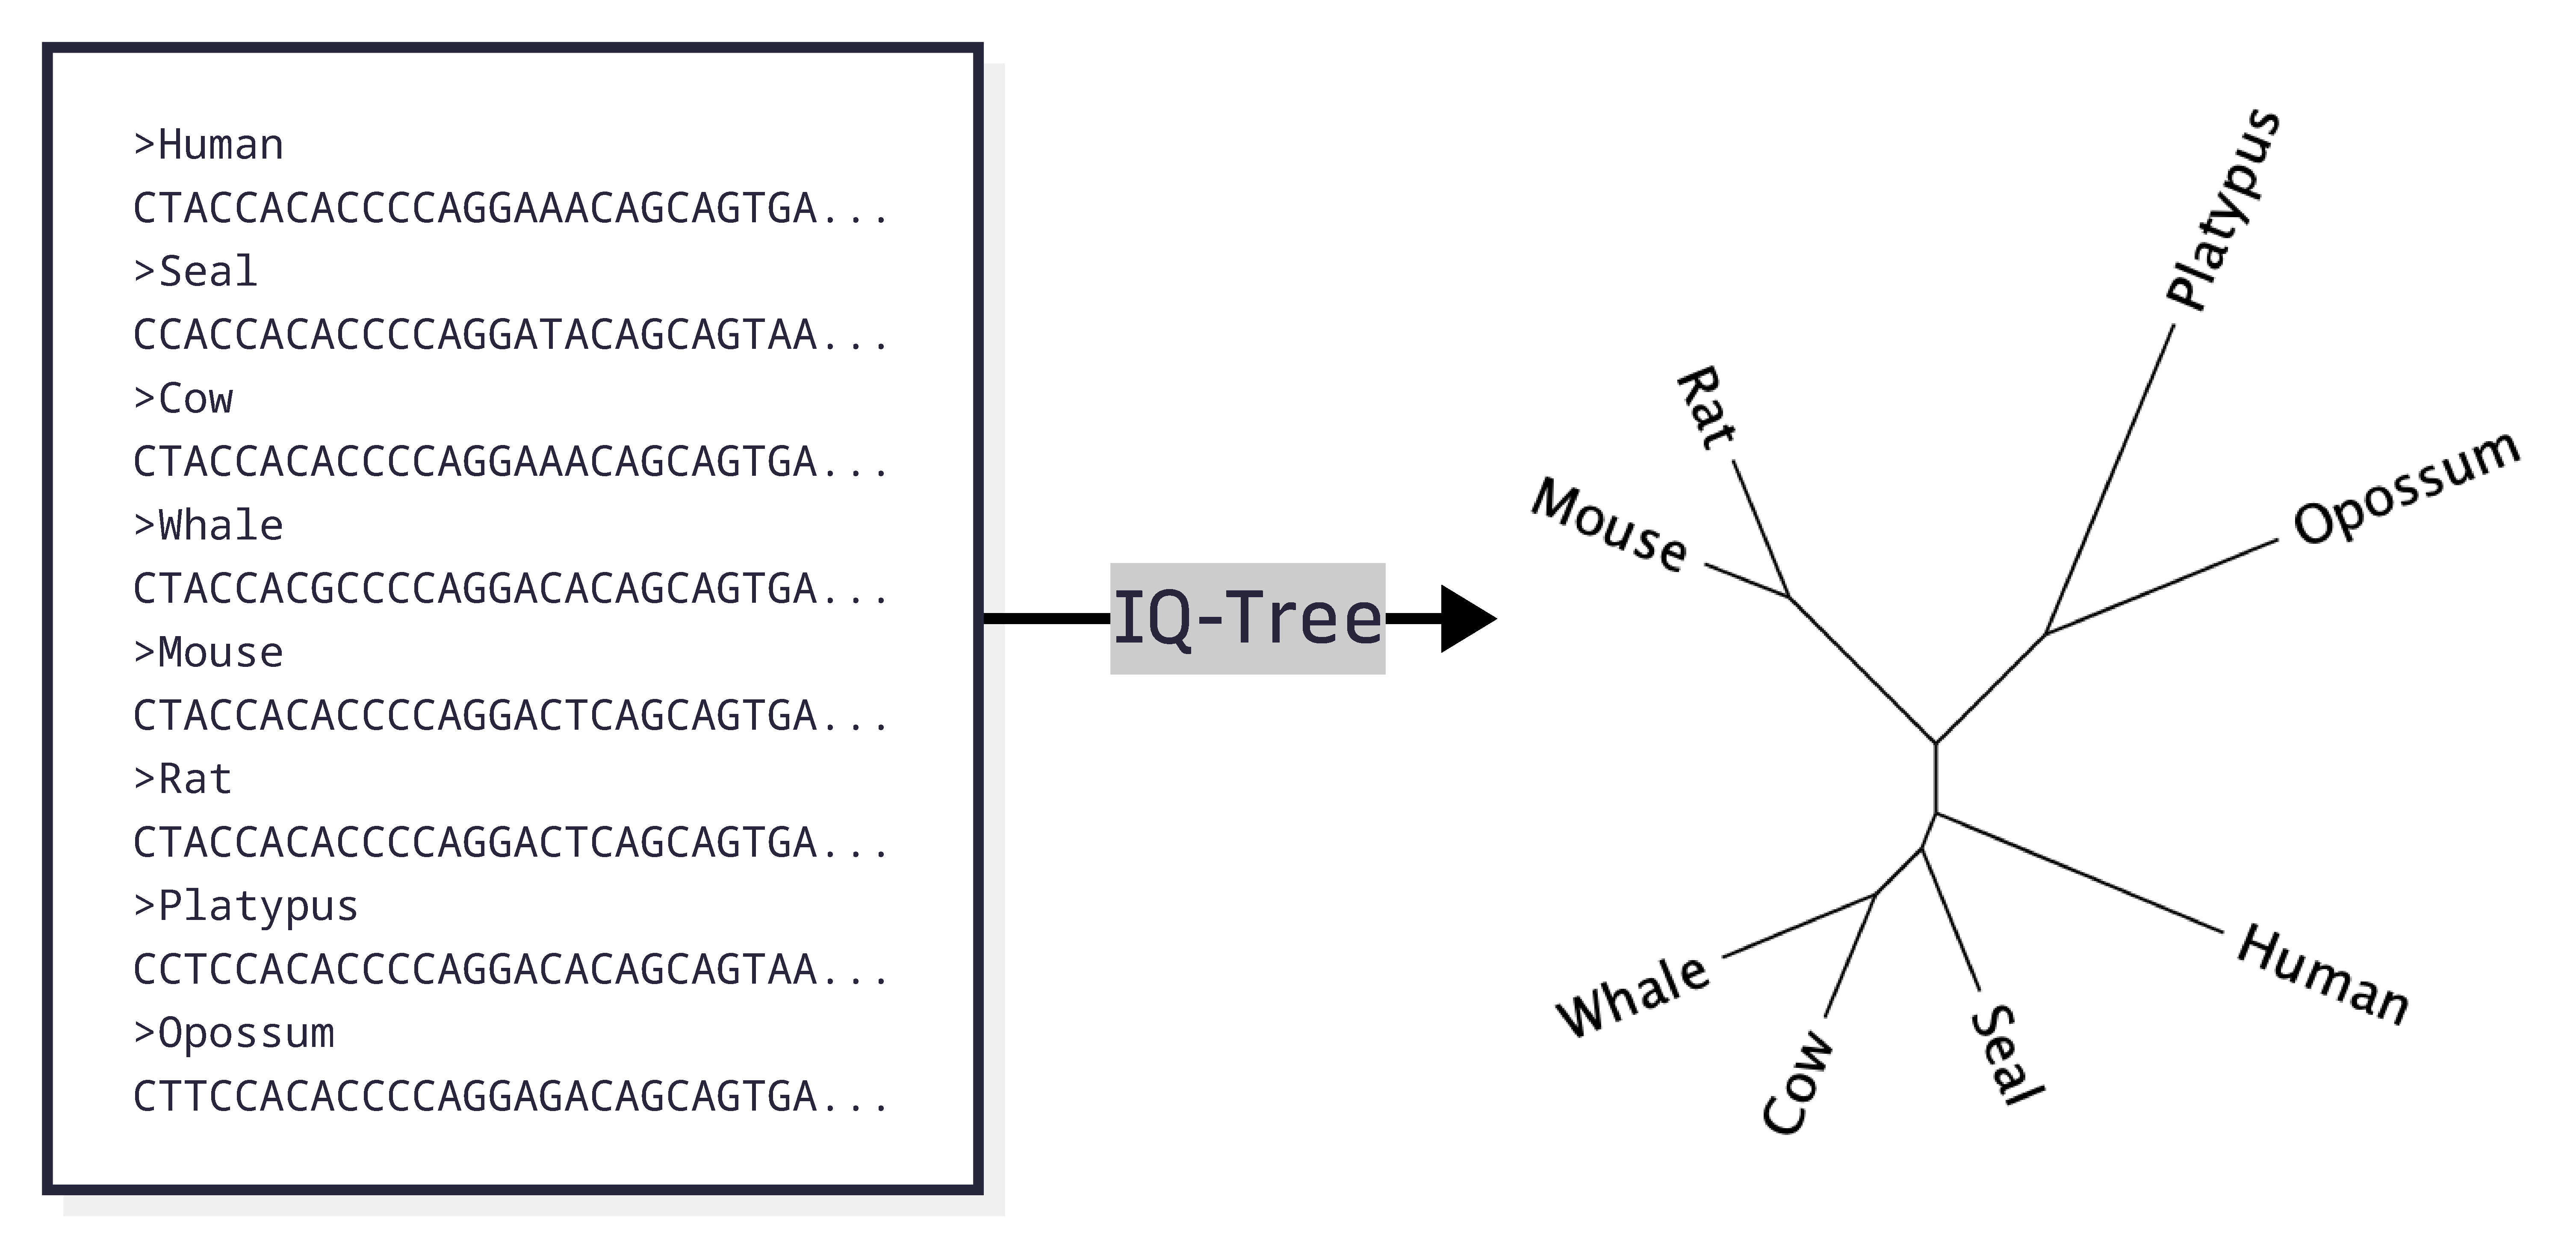
\includegraphics[scale=0.14]{iq_tree_basic_diagram.pdf}
    \end{centering}
    \pause
    \begin{itemize}
        \item Resulting tree that is best explained by data, i.e. maximum likelihood $\mathbb{P}(\text{aligned sequences}~\vert~\text{tree, model of evolution})$
        \item Phylogenetic assumptions? Phylogenetic information present in alignment?
    \end{itemize}
\end{frame}

\begin{frame}
    \frametitle{Quartets and Likelihood Mapping}
    \begin{itemize}
        \item Assess whether the alignment is suitable for a phylogenetic reconstruction.\pause
        \item \alert{Can a tree be reliably resolved, even if its (quartet) subtrees cannot?}
    \end{itemize}

    \pause
    For a quartet $\{ A, B, C, D\}$ of leaves, there are only $3$ possible tree topologies (up to isomorphism):

    \centering
    \begin{tabular}{lccc}
        &
        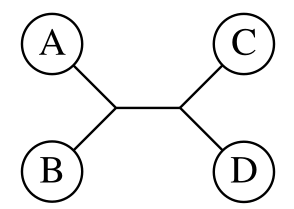
\includegraphics[scale=0.3]{quartet_topology-1.png}
        &
        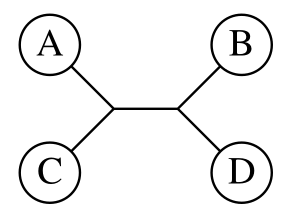
\includegraphics[scale=0.3]{quartet_topology-2.png}
        &
        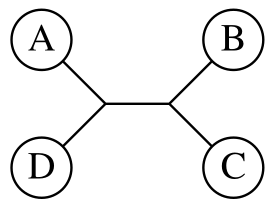
\includegraphics[scale=0.3]{quartet_topology-3.png}
        \pause
        \vspace{1em}
        \\
        & $\Downarrow$ & $\Downarrow$ & $\Downarrow$
        \vspace{1em}
        \\
        resulting likelihoods
        &
        $L_1$
        &
        $L_2$
        &
        $L_3$ 
        \vspace{1em}
        \\
        posteriors
        &
        $p_1 = \frac{L_1}{L_1 + L_2 + L_3}$
        &
        $p_2 = \frac{L_2}{L_1 + L_2 + L_3}$
        &
        $p_3 = \frac{L_3}{L_1 + L_2 + L_3}$

    \end{tabular}
\end{frame}

\begin{frame}
    \frametitle{Quartets and Likelihood Mapping Continued}
    \[
        p_i \geq 0 \text{ and } p_1 + p_2 + p_3 = 1 \implies (p_1, p_2, p_3) \in \Delta^2 = \left\{  (x_0, x_1, x_2) \in \mathbb{R}^3 \mid x_i \geq 0, \sum_{i=0}^2 x_i = 1 \right\}
    \]
    \centering
    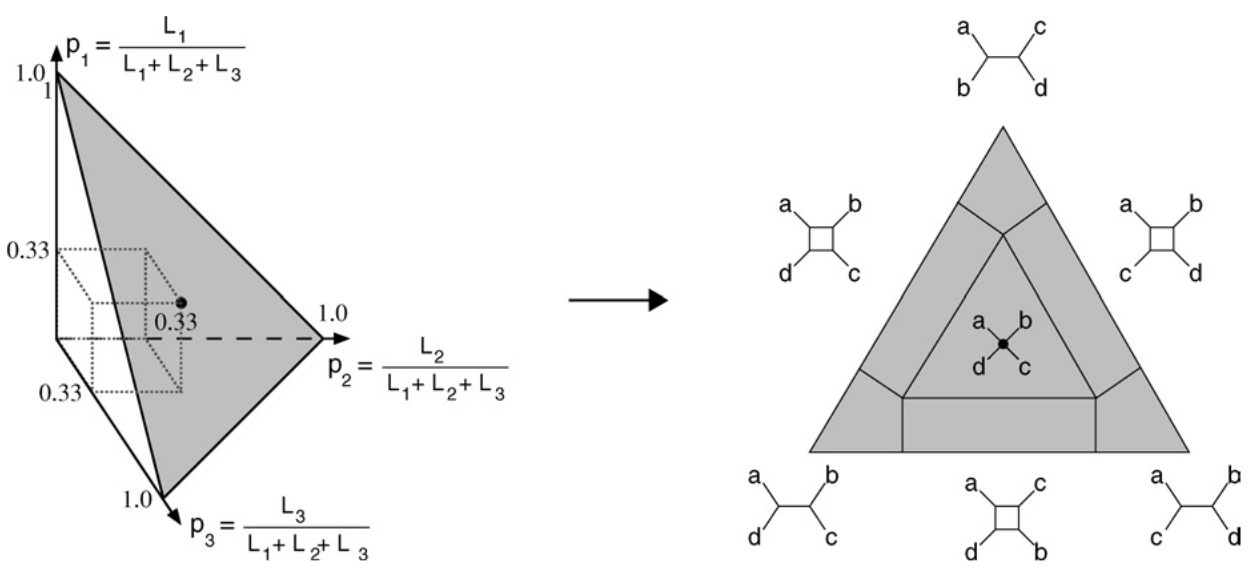
\includegraphics[scale=0.25]{simplex_visualisation.png}
\end{frame}

\begin{frame}[fragile]
    \frametitle{Likelihood Mapping Diagrams}

    \begin{columns}
        \begin{column}{0.5\textwidth}
            \centering
            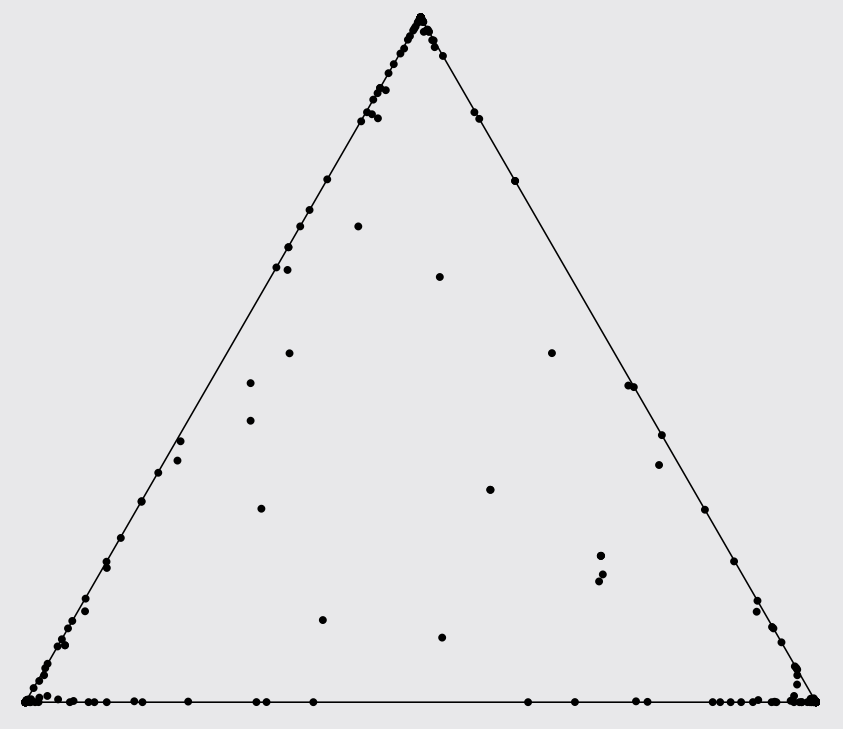
\includegraphics[scale=0.25]{likelihood_diagram.png} 
        \end{column}
        \begin{column}{0.5\textwidth}
            \centering
            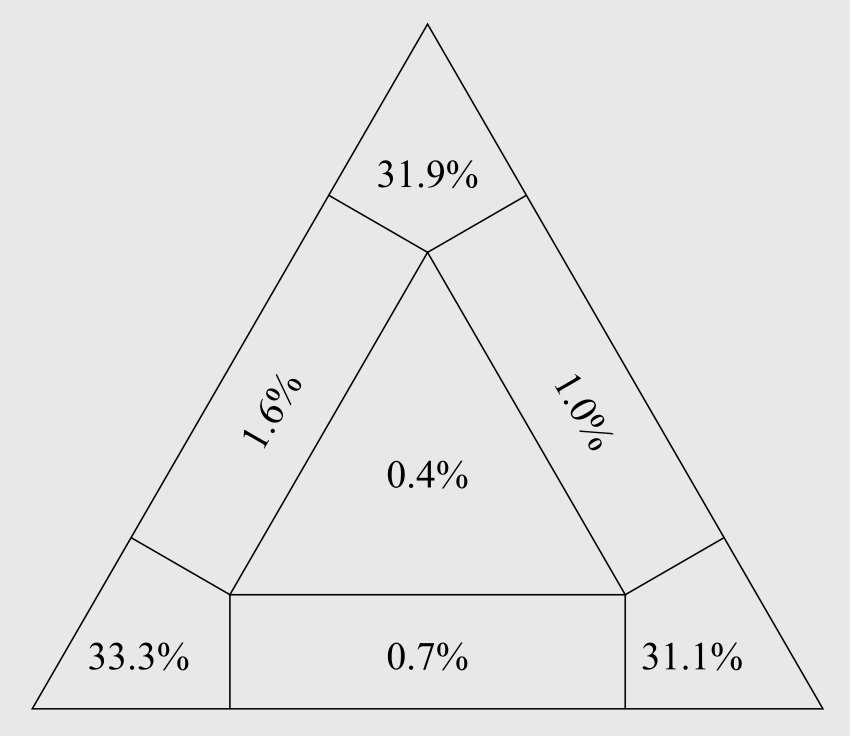
\includegraphics[scale=0.25]{likelihood_diagram_percentages.png} 
        \end{column}
    \end{columns}
    \pause
    \vspace{1em}
    Heuristic: more than $20 - 30\%$ outside of the corners $\implies$ data not reliable for phylogenetic inference
\end{frame}

\begin{frame}[fragile]
    \frametitle{Likelihood Mapping Summary}
    \footnotesize
    \centering
    \begin{semiverbatim}
Quartet resolution per sequence (phylogenetic information):

      #quartets   resolved           partly          unresolved  name
-----------------------------------------------------------------------------
   1      276    271 ( 98.19)       5 (  1.81)       0 (  0.00)  HIV1groupO
   2      291    283 ( 97.25)       8 (  2.75)       0 (  0.00)  SIVcpzUS
   3      289    272 ( 94.12)      13 (  4.50)       4 (  1.38)  SIVcpzGAB
   4      295    274 ( 92.88)      17 (  5.76)       4 (  1.36)  aU09127
   5      286    273 ( 95.45)       9 (  3.15)       4 (  1.40)  gU27426
   6      267    255 ( 95.51)      12 (  4.49)       0 (  0.00)  gU27445
   7      263    256 ( 97.34)       7 (  2.66)       0 (  0.00)  cAF067158
   8      289    269 ( 93.08)      20 (  6.92)       0 (  0.00)  cU09126
   9      297    288 ( 96.97)       9 (  3.03)       0 (  0.00)  dU27399
  10      282    271 ( 96.10)      11 (  3.90)       0 (  0.00)  dU43386
  11      288    283 ( 98.26)       3 (  1.04)       2 (  0.69)  bL02317
  12      292    283 ( 96.92)       9 (  3.08)       0 (  0.00)  bAF025763
  13      301    297 ( 98.67)       2 (  0.66)       2 (  0.66)  bU08443
  14      284    277 ( 97.54)       7 (  2.46)       0 (  0.00)  bAF042106
-----------------------------------------------------------------------------
         1000    963 ( 96.30)      33 (  3.30)       4 (  0.40)
    \end{semiverbatim}   
\end{frame}

\begin{frame}[fragile]
    \frametitle{Problem Statement}
    Not all quartets might be equally informative.
    Some quartets are more likely to be resolved correctly than others.
    Example:
    \begin{columns}
        \begin{column}{0.3\textwidth}
            \begin{semiverbatim}
                >A_1
                ACAGT
                >A_2
                ACAGT
                >A_3
                ACAGT
                >B
                TGAGT
            \end{semiverbatim}
        \end{column}
        \begin{column}{0.3\textwidth}
            \begin{align*}
                A_1 = A_2 = A_3 \implies \\
                 (p_1, p_2, p_3) = (1/3, 1/3, 1/3)
            \end{align*}
        \end{column}

        \begin{column}{0.3\textwidth}
            sadf
        \end{column}
\end{columns}

\end{frame}


\begin{frame}
    \frametitle{Implementation Details}
    \begin{columns}
        \begin{column}{0.5\textwidth}
            \begin{itemize}
                \item C++ (\texttt{-std=c++17})
                % cloc alignment main model tree utils
                \item $\geq 80000$ lines of code
                \item CMake Build System
                \item Dependencies:
                \begin{itemize}
                    \item Eigen3
                    \item Boost
                    \item MPI (Message Passing Interface)
                \end{itemize}
                \item Git repository hosted on GitHub
                \item Documentation with Doxygen
                \item Test scripts included
                \item CI script running on GitHub Actions
            \end{itemize} 
        \end{column}
        \begin{column}{0.5\textwidth}
            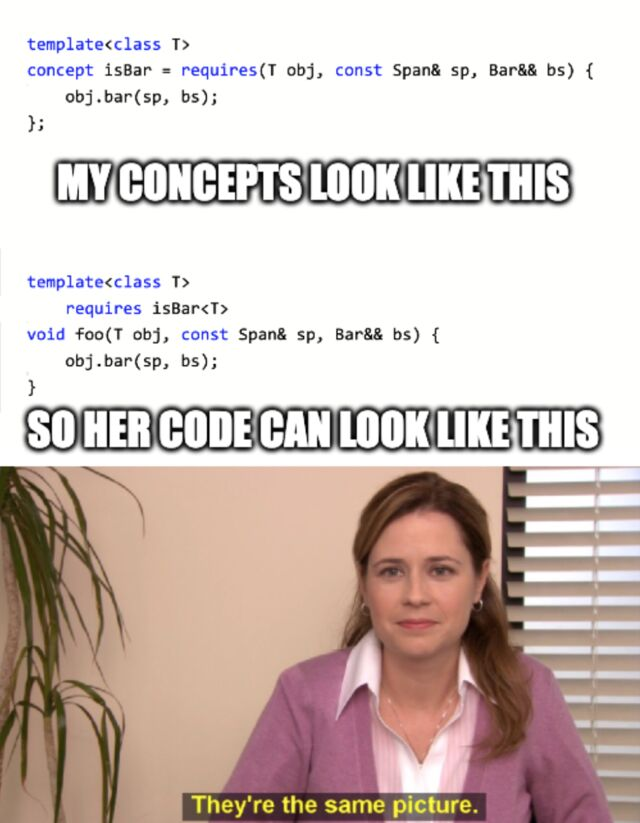
\includegraphics[scale=0.54]{my-concepts-look-like-this.jpg} 
        \end{column}
    \end{columns}
\end{frame}

\begin{frame}[standout]
    Thank you! 
\end{frame}

\end{document}